%\pdfoutput=1
\documentclass[oneside,12pt]{article}%
%\usepackage[cp852]{inputenc} % pouľito v případě jiného kódování
% aktuální kódování: ISO Latin 2 (ISO 8859-2)
\usepackage{dipp}
\usepackage{eurosym}

\usepackage[]{graphics}
\graphicspath{ {/home/zahrada/Dropbox/bachelor_thesis_VM/thesis-vm/img/} }
\linespread{1.5}
\begin{document}

\def\,{\penalty10000\hskip.25em}

\pagestyle{headings}

\pagenumbering{gobble}
\bakalarska

\titul{Vladcina BP}{Vladislava Muselikova}{--}{Brno 2015}


\prohlasenizena{V~Brně dne \today}

\podekovani{Pod\v{e}kov\'{a}n\'{i}...}

\abstract{The Bachelor thesis Supplier evaluation system of the wood processing enterprise in the region of the CR, the SK, HU and AT deals with analysis of the current supplier evaluation system in IKEA Industry company in Malacky. The theoretical part is based on literature review and contains description of the purchasing process and methodology for selection and evaluation of suppliers. The practical part is devoted to the analysis of the Supplier Classification in IKEA and gives suggestions for specific improvements for the system in IKEA Industry Malacky, which deals with purchasing and processing of the raw material.}{key words...}

\newpage

\abstrakt{Bakal\'{a}\v{r}sk\'{a} pr\'{a}ce Syst\'{e}m hodnocen\'{i} dodavatel\r{u} v regionu \v{C}R, SK, HU a AT se zab\'{y}v\'{a} anal\'{y}zou sou\v{c}asn\'{e}ho syst\'{e}mu hodnocen\'{i} v IKEA Industry v Malack\'{a}ch. Teoretick\'{a} \v{c}\'{a}st je zalo\v{z}en\'{a} na liter\'{a}rn\'{i} re\v{s}er\v{s}i a obsahuje popis n\'{a}kupn\'{i}ho procesu a metody pro hodnocen\'{i} a v\'{y}b\v{e}r dodavatel\r{u}. Praktick\'{a} \v{c}\'{a}st je zam\v{e}\v{r}ena na anal\'{y}zu Klasifikace Dodavatel\r{u} ve spole\v{c}nosti IKEA a nab\'{i}z\'{i} mo\v{z}n\'{a} specifick\'{a} \v{r}e\v{s}en\'{i} pro syst\'{e}m v z\'{a}vod\v{e} IKEA Industry v Malack\'{a}ch, kter\'{y} se zab\'{y}v\'{a} n\'{a}kupem a zpracov\'{a}n\'{i}m surov\'{e}ho materi\'{a}lu.}{klicovy pizdec}



\obsah
\pagenumbering{arabic}
\setcounter{page}{7}
\kapitola{Introduction}

A very basic part of business management is the purchasing function. Supply chain management and strategic sourcing have been one of the fastest growing area of management, particularly last ten years. Enterprises, especially in post-soviet countries, are aware of this fact, nevertheless they still tend to put more effort into the process of selling, but some of them necislovated to realize, that with studied system of the purchase they could save more money than in a case of high sells with extra expenses when purchasing the material. Within the purchasing function one of the prime responsibilities is the selection and evaluation of suppliers. The awareness of importance of selection of suppliers is dated to early forties, when Lewis (1943) stated: “It is probable that of all the responsibilities which may be said to belong to the purchasing officers, there is none more important than the selection of a proper source. Indeed, it is in some respects the most important single factor in purchasing”. \par
In most industrial companies raw material represents the largest percentage of the cost. For instance, in wood processing industry, it can be about 70\% of the total product cost. Therefore the selection of the right supplier is absolutely crucial.\par
To successfully assess possible suppliers the company must take into account many qualitative and quantitative criteria. We can take these factors and group them and get different approaches. These, in literature suggested, approaches can be difficult to handle in reality and company managers can overcome many difficulties when they find out that the specific system is not applicable and should consider that certain level of flexibility is necessary.



\begin{table}
  \scalebox{0.7}{
  \begin{tabular}{c|c}
    Supplier & Points \\ \hline
    A        & 20     \\
    B        & 15     \\
    C        & 24     \\
    D        & 14     \\
    E        & 14     \\
    F        & 19     \\
    G        & 19     \\
    H        & 18     \\
    I        & 21     \\
    J        & 18     \\
    K        & -      \\
    L        & 16     \\
    M        & -      \\
    N        & -      \\
    O        & 17

  \end{tabular}
  }
  \caption{popis}
\end{table}


\begin{table}
  \parbox{.45\linewidth}{
  \centering
  \begin{tabular}{ccc}
    \hline
    a&b&c\\
    \hline
  \end{tabular}
  \caption{Foo}
  }
  \hfill
  \parbox{.45\linewidth}{
  \centering
  \begin{tabular}{ccc}
    \hline
    d&e&f\\
    \hline
  \end{tabular}
  \caption{Bar}
  }
\end{table}

\kapitola{Objectives}
The main objective of this thesis is to analyze current system of supplier evaluation in enterprise Ikea Industry in Malacky and discuss eventual improvements, based on literature review and practical evaluation.\par
Theoretical part of the thesis is based on literature review and is divided into two main chapters: Purchase and Suppliers. The Purchase chapter includes details about Supply Chain Management as well as about the purchasing process and single steps of the process. Follow-up chapter includes description of the supplier selection and evaluation system, criteria involved in this process and the most important and frequently used methods for supplier selection.\par
The IKEA Industry Group, formerly Swedwood Group, is a fully integrated international industrial group of IKEA. There are two focuses of the production in the enterprise IKEA Industry in Malacky. Firstly it is the produce of chipboard from the raw materials as raw wood and wood chips. Secondly it is the manufacture of furniture components – parts which are made of the chipboard and afterwards send to the retail stores mainly in Europe.\par
Ikea Industry is currently dealing with a change of system of suppliers. The old system was designed by a responsible person within the enterprise and the new one comes as centrally designed system from Sweden. So called Supplier classification is only applicable for evaluation of Home Furnishing Suppliers and Components suppliers so the IKEA Industry is almost completely excluded as the main object of purchase is the raw material.\par
Practical part of the thesis deals with analyzing of the data provided by IKEA and actual visit of few suppliers. It contains description of the company and the enterprise, specific criteria, typical for IKEA or IKEA Industry, analyze of the past and current system and the data. The data of the purchasing history are transferred within Excel tables and form comprehensive overview of the situation. Based on the data and personal meetings there is a summary of problems and formulated improvements and suggestions for this specific situations.



\kapitola{Methodology}
The theoretical part mainly includes information based on extensive study of academy textbooks, both Czech and foreign. The work is further supported with information and statistical data found in online academic journals and scholars. Last but not least, the thesis contains. \par
As the prime sources for this part of the thesis were studied online articles from academic journals supported with extensive study of academic textbooks, both Czech and foreign. The thesis also encompasses statistical data taken from academic journals, dissertation and diploma works. \par
Practical part of the thesis deals with analyzing of the data provided by IKEA and actual visit of few suppliers. It contains description of the company and the enterprise, specific criteria, typical for IKEA or IKEA Industry, analysis of the past and current system and the data. The data of the purchasing history are transferred within Excel tables and form comprehensive overview of the situation. Based on the data and personal interviews there is a summary of problems and formulated improvements and suggestions for this specific situations. These problems were further compared with the literature review.

\kapitola{Literature Review}
The following part of the bachelor thesis deals with the description of the purchasing function in general and with the focus on the suppliers – criteria for selection, selection methods and evaluation.

\sekce{Role of the purchasing management within the Supply chain management}
To describe these two fundamental terms we have to consider the scope and focus. Some academic specialists see these as practically the same (Stuart, 1997), while some see SCM as about developing relationship with suppliers (Giunipero and Brand, 1996) and others say that good supplier management is not enough and there is an additional requirement for a wider, more integrated, all – encompassing perspective which embrace all the processes from sourcing to merchandising (Davis, 1993). Monczka et al. (2005) gives a comprehensive definition: “SCM is a strategic approach to planning for and acquiring the organization’s current and future needs through effectively managing the supply base, utilizing a process orientation in conjunction with cross-functional teams to achieve the organizational mission.” \par
To simplify this topic and relate it to the level of bachelor thesis, the SCM term will not be used and purchasing management will be taken as superior term to supplier management, which involves the selection, evaluation and relationship with the suppliers.\par
The purchasing function traditionally encompasses the process of buying. It involves determining of the purchasing needs, selecting the supplier, arriving at a proper price, specifying terms and conditions, issuing the contract or order, and following up to ensure proper delivery and payment. (van Weelen, 2009)

\begin{enumerate}
  \item Supply continuity – traditional role of the purchasing function is the satisfying of the requirements of the internal customers. Purchasing supports operations within the purchase of raw materials, components and others. The support of the physical distribution is also in the responsibilities of the purchasing function. Key to the smooth flow is in the following  steps:
  \begin{itemize}
    \item   At the right place - the costs will be minimized, only in the case of optimizing the price
    From the best source – qualities as reliability, efficiency and dealing with queries as the example of after cooperation
    \item Of the right quality – to low quality can result in high wastage of materials, extra labor expenses, increased machine time and wear and mainly spoilt production
    \item In the right quantity
    \item At the right time - this point is closely connected to the right quantity, so there is limited chance of running out of stock and minimalizing the expenses for long stocking.
  \end{itemize}



  \item Manage the purchasing process efficiently and effectively – purchasing management must continuously look for employees with developed skills and constantly try to improve the transactional level work through efficient purchasing systems. The objective is completed if following internal operations are managed:
    \begin{itemize}
    \item Optimal staffing levels
    \item Keeping the administrative calculations
    \item Professional training for the staff
    \item Accounting transparency – system which is easy to use and follow
    \end{itemize}


  \item Develop supply base management – selecting, developing and maintaining the supply, so called supply base management. The key focuses are:
  \begin{itemize}
    \item Selection of competitive suppliers which have potential for excellent performance and development of the relationship with these suppliers,
    \item Improving current suppliers
    \item Developing suppliers which are not competitive, if possible
  \end{itemize}

  \item Develop aligned goals with internal functional stakeholders – improving the communication within the company as well as with the suppliers and big internal customers – stakeholders. This, for example, includes communication between marketing and purchasing department, when marketing spends a great deal on promotion, purchasing must ensure that the pricing is competitive. Other functional groups are: manufacturing, engineering, technology and finance.

  \item Support Organizational Goals and Objectives – purchasing may directly affect overall performance and for this reason must be concerned with the organizational directives. Purchasing management can work with suppliers to extend/reduce delivered quantities and other steps which can influence the performance.

  \item Develop Integrated Purchasing Strategies – which supports company plans. Purchasing was/is often seen as a tactical support function rather than the part of corporate planning and executive management did/does not recognize the benefits of well-thoughtout purchasing. These two factors are quickly changing and purchasing is usually actively involved in strategic planning. The areas which are regularly reviewed are:
  \begin{itemize}
    \item Market trends (price, changes in suppliers)
    \item Critical materials which are needed especially during new product development
    \item Supply options including the globally competitive supply base suitable for the company
  \end{itemize}

\end{enumerate}
  One of the objectives of purchasing is ensuring the purchasing process which includes steps, which must be followed when company requires some product, material or service. The process includes step from the initial phase of identification of the problem to the payment and evaluation of the performance. The following process shown in the Fig. 1 was designed by van Weele (2009):

% fig 1

\begin{figure}[ht!]
  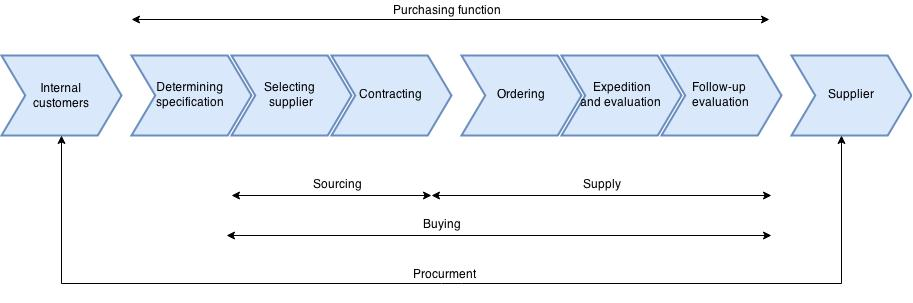
\includegraphics[width=1\textwidth]{purchase_process.jpg}
  \caption{Purchasing process activites (van Weele, 2009)}
\end{figure}

As mentioned, purchasing decision making directly influence the profitability of the company. With the progress and more focus from the public, companies have to take into account not only their own interests, but also government regulations or environmental concerns. In the Fig. 1 is shown the factors which are involved in purchasing making decision.

\begin{figure}[ht!]
  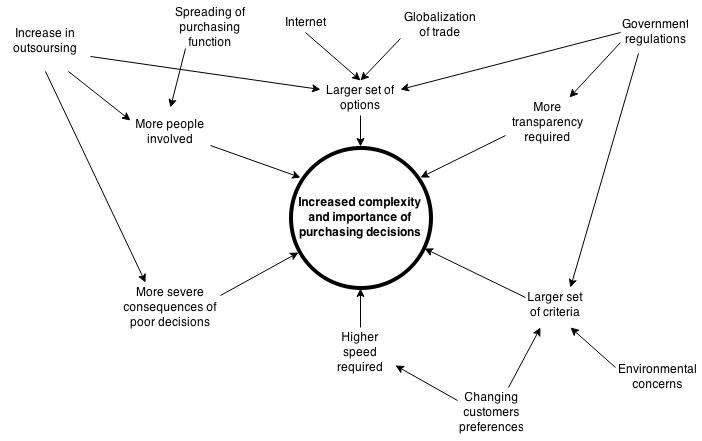
\includegraphics[width=1\textwidth]{complexity.jpg}
  \caption{Impact of developments on the complexity of initial purchasing decisions (de Boer, 1998)}
\end{figure}

Current trends shows the use of decision models in purchasing implies that the mathematical nature of the models is incompatible with the highly emotion and intuition driven practice of purchasing decision-making used in the past.

\sekce{Suppliers}
As mentioned before, supplier management is the key part of the strategy management which can be completely crucial for the company’s profit. Nevertheless suppliers are not equal, but this does not mean there is only one suitable supplier. Current trend is to have so called strategy supplier – supplier that is very responsible, but the rate of dependency is not very high. And the supplier is able to cover more than 30% of the company demand.
There are further classifications and divisions of the suppliers which serve for both, evaluation and selection. Monczka et. al (2007) suggests to define the suppliers as follows:

\begin{itemize}
  \item Manufacturer vs. distributor, the choice is based on these criteria: (1) the size of the purchase; (2) the manufacturer’s policies regarding direct sales; (3) the storage space available at the purchaser’s facility; and (4) the extent of services required. In case of IKEA Industry would be more appropriate to consider suppliers from the private and state sector
  \item Local or national or international suppliers – in the wood industry firms consider cost of transport, possible forest production and some companies take into account environmental issues. The issue is sometimes limited to the fact that demanded kind of wood grows only in certain areas.
  \item Large or small suppliers – some purchases prefer to focus on small suppliers as they are more willing to cooperate and discuss the conditions. Also if the firm wants to reduce the level of dependency it is convenient to extend the portfolio of suppliers.
  \item Multiple or Single Sourcing – surely, the trend goes towards reducing the number of suppliers, however, the assurance of supply is higher in the case of multiple sourcing.
  Innovative or conservative suppliers
\end{itemize}


\sekce{Supplier selection process}
For the matter of supplier selection process and methodology, there are rich sources in terms of conceptual and empirical research and decision support methods for purchasing managers but none of these articles actually has studied how managers choose suppliers in practice (Verma, 1998) and there is no universal or best way to evaluate and select suppliers. For this reason the thesis deals with literature review and the practical part will include the description of actual supplier selection in Ikea Industry. Following steps were further discussed by Monczka et al. (2005):


\begin{description}
  \item[Step 1: Recognize the need for supplier selection] \hfill \\
  This usually means realizing that there is a requirement to evaluate and select a supplier to cover the gaps in the company progress. Responsible person is a purchasing manager who might begin the process with anticipation of a future purchase demand. The recognition of a need of evaluation and selection new suppliers can come in different ways. This may include new product development, the end of contract, poor supplier performance, extension into new markets and others.

  \item[Step 2: Identify key sourcing requirements] \hfill \\
  The criteria of selection for specific supplier differ with every supplier. In our case, the IKEA Industry have suppliers from different countries, this in practice means, that some suppliers cannot compete with the price of transport, but they have other qualities which make them competitive. Although the criteria are not constant, certain factors should be involved in every evaluation: cost, quality and delivery performance.

  \item[Step 3: Determine Sourcing Strategy] \hfill \\
  The company can and should have different approaches to the sourcing with different suppliers. Companies usually prepare some initial strategy with many different decisions, however these often need a change as a result of conditions during actual selection – market conditions, purchaser preferences or corporate objectives. Among decisions which need to be done are:
  \begin{itemize}
  \item Single versus multiple supply sources
  \item Short-term versus long-term purchase contracts
  \item Selecting suppliers that provide design support versus those that lack design capability
  \item Full-service versus non-full-service suppliers
  \item Domestic versus foreign suppliers
  \item Expectation of a close working relationship versus arm’s-length purchasing
  \end{itemize}
  The common experience says, that single sourcing is not appropriate and in case of IKEA it is an extreme truth – the whole IKEA has more than 5000 suppliers (IKEA). Other decisions differ supplier from supplier


  \item[Step 4: Identify Potential Supply Sources]
  As there are different sourcing strategies, there are also different ways how to actually search new potential suppliers. The intensity of the search is influence by several variables as how well existing suppliers can satisfy buyers, strategic importance or technical background. The most common and valuable sources where to search for suppliers are:
  \begin{itemize}
    \item Current suppliers – purchaser can easily identify new purchase requirements when looking at current suppliers. Selecting existing supplier for new purchase is appealing, on the other hand, managers may not know, if there are better options without searching other options.
    \item Sales Representatives, Information Databases – are sometimes available for purchase from external parties, especially for foreign sources
    \item Experience, Trade Journals, Trade Directories, Trade Shows ,Second-Party or Indirect Information
    \item Internet – belongs to current trend and is considered as the quickest way for searching new suppliers. The Internet is considered to be good for searching alternatives and in initial steps of searching.

  \end{itemize}
  There are also involved employees from different departments, who should be equally interested and undertake the same level of the risk. There are: users of the products or service, influencers, deciders, approvers, buyers and purchaser. All these roles are important for security of the subjectivity of the process.


  \item[Step 5: Limit Suppliers in Selection Pool]

  The step basically involve the preselection of the suppliers based on criteria which are essential for the certain company. In case of IKEA, there is directive called IWAY and potential suppliers must be IWAY approved to be consider as supplier for further analysis. As critic criteria are also considered the price and quality. In this case supplier may use the help of ISO standardization, e.g. ISO 9001. The step is further discuss in the section of pre-qualifying of the suppliers.

  \item[Step 6: Determine the Method of Supplier Evaluation and Selection]
  Once the initial cuts has been done, the buyer must decide how to evaluate the rest, to reduce the number to the final group. There are several methods for the supplier selection and some of these methods are described in the following section 3.2.3.5. In practice this can mean also visit of the supplier, evaluation of supplier provided information or information provided by a third part and use of preferred suppliers.

  \item[Step 7: Select Supplier and Reach Agreement]
  The final step of the evaluation and selection process is to select the supplier(s) and reach a contract agreement. The activities associated with this step can vary widely depending on the purchase item under consideration. For routine items, this may simply require notifying and awarding a basic purchase contract to a supplier. For a major purchase, the process can become more complex. The buyer and seller may have to conduct detailed negotiations to agree upon the specific details of a purchase agreement. Also personal audits based on the evaluation are part of this step.

\end{description}


\sekce{Decision criteria}
Decision criteria are set of requirements which must be completed by the supplier part and the list of criteria is used for assessment. The criteria might be assigned different weight according the type of selection system. \par
Little bit outdated, bit still very informative work was published by Dickson (Dickson, 1966). He sent 273 questionnaires to managers of leading companies in the USA and Canada and asked to mark criteria which are the most seminal in the decision-making process. In his book he stated, that it is quite easy to abstract list of 50 distinct criteria and for his study he chose 23 which were constantly repeating in the surveys. These factors are shown in the Tab 1. bellow in order of importance. We have to consider the fact, that this list was revealed in the sixties and the table would little bit differ with diverse products, for this reason the Tab 1. Also includes the order suggested by Weber (1991) The most significant difference is spot in geographical location as nowadays the logistics method of stocking just-in-time (JIT) is very popular and suppliers are required to deliver on time. There are another reasons, as environmental issuer, which are not included as the significance in 1966 was not high.


\begin{table}[h]
  \tiny
  \begin{tabular}{lll}
    \multicolumn{2}{c}{Rank}                                         &                                                                                   \\ \cline{1-2}
    \multicolumn{1}{l|}{Dickson} & \multicolumn{1}{l|}{Weber et al.} & Criteria                                                                          \\ \hline
    \multicolumn{1}{l|}{1}       & \multicolumn{1}{l|}{3}            & Quality                                                                           \\
    \multicolumn{1}{l|}{2}       & \multicolumn{1}{l|}{2}            & Delivery                                                                          \\
    \multicolumn{1}{l|}{3}       & \multicolumn{1}{l|}{10}           & Performance History                                                               \\
    \multicolumn{1}{l|}{4}       & \multicolumn{1}{l|}{23}           & Warranties and Claim Policies                                                     \\
    \multicolumn{1}{l|}{5}       & \multicolumn{1}{l|}{4}            & \begin{tabular}[c]{@{}l@{}}Production Facilities \\ and Capabilities\end{tabular} \\
    \multicolumn{1}{l|}{6}       & \multicolumn{1}{l|}{1}            & Net Price                                                                         \\
    \multicolumn{1}{l|}{7}       & \multicolumn{1}{l|}{6}            & Technical Capability                                                              \\
    \multicolumn{1}{l|}{8}       & \multicolumn{1}{l|}{9}            & Financial Position                                                                \\
    \multicolumn{1}{l|}{9}       & \multicolumn{1}{l|}{16}           & \begin{tabular}[c]{@{}l@{}}Bidding Procedural \\ Compliance\end{tabular}          \\
    \multicolumn{1}{l|}{10}      & \multicolumn{1}{l|}{18}           & Communication System                                                              \\
    \multicolumn{1}{l|}{11}      & \multicolumn{1}{l|}{8}            & Reputation and Position in Industry                                               \\
    \multicolumn{1}{l|}{12}      & \multicolumn{1}{l|}{21}           & Desire for Business                                                               \\
    \multicolumn{1}{l|}{13}      & \multicolumn{1}{l|}{7}            & Management and Organization                                                       \\
    \multicolumn{1}{l|}{14}      & \multicolumn{1}{l|}{14}           & Operational Controls                                                              \\
    \multicolumn{1}{l|}{15}      & \multicolumn{1}{l|}{11}           & Repair Service                                                                    \\
    \multicolumn{1}{l|}{16}      & \multicolumn{1}{l|}{12}           & Attitude                                                                          \\
    \multicolumn{1}{l|}{17}      & \multicolumn{1}{l|}{20}           & Impression                                                                        \\
    \multicolumn{1}{l|}{18}      & \multicolumn{1}{l|}{13}           & Packaging Ability                                                                 \\
    \multicolumn{1}{l|}{19}      & \multicolumn{1}{l|}{17}           & Labor Relations Records                                                           \\
    \multicolumn{1}{l|}{20}      & \multicolumn{1}{l|}{5}            & Geographical Location                                                             \\
    \multicolumn{1}{l|}{21}      & \multicolumn{1}{l|}{22}           & Amount of Past Business                                                           \\
    \multicolumn{1}{l|}{22}      & \multicolumn{1}{l|}{15}           & Training Aids                                                                     \\
    \multicolumn{1}{l|}{23}      & \multicolumn{1}{l|}{19}           & Reciprocal Arrangements
  \end{tabular}
\end{table}

Later, Lehman and O’Shaugnessy (1982) suggested in their study to form groups of factors: performance criteria, economic criteria, integrative criteria and adaptive criteria - extent to which buying firm may have to adapt its plans to accommodate uncertainty about the capability of the supplier (Vokurka et al., 1996) The literature related to the problem of criteria in the supplier selection problem is very rich. As another example how we can look at criteria was distinguished by Barbarosoglu and Yazgac (1997) and the work suggests to form groups of three principle criteria:

  \begin{itemize}
    \item The performance of the supplier
    \item The business structure/manufacturing capability of the supplier
    \item The quality of the products
  \end{itemize}

Each criteria group have many sub-criteria, but the description go beyond the frame of the thesis.

\podsekce{Weights put on different criteria}
After identifying factors which are important for specific commodity, the company management is supposed to assign weights to each criteria and sub-criteria which are subordinate. This reflect relative importance of each criteria. This step also include the way how will be each category assessed. In case of IKEA, they have chosen the method of goals. In each category there is defined goal position and wished position. Wished position shows the best possible results in the category. Category goal is a position which can be reached by suppliers in case of outstanding performance. Usually this means, that the best supplier is positioned on the level of category goal or slightly above. If the supplier has better performance than is the wished position, it mean there might be some mistake in the supplier management and this business cannot be profitable. The scoring in sub-criteria is normally averaged and the result stands for the result of the category. As very suitable method for weight assignment is AHP, described further in the chapter 3.2.3.5.1.

\sekce{Suppliers selection and evaluation methods}

The supplier selection was supposed to be a matter of straightforward process, but later the approach had to changed due to difficulties such as (1) growing number of potential suppliers; (2) growing number of attributes; (3) increasing number of situational contexts that affect appropriateness of specific supplier attributes; and (4) difficulty in identifying and defining supplier selection parameters (Altinoz et al., 2010). \par
There is a large number of existing decision making methods whom main goal is to assist in supplier selection. Both, qualitative and quantitative factors are involved. As previously mentioned the contemporary supply management is to maintain long term partnership with suppliers and rely on fewer of them. This thesis differ terms system and method. The system stands for the approach and the method describes models which are suitably used for the certain system. Therefore there are three systems: categorical system, weight point system and cost based system. In the Figure 3. there are shown advantages and disadvantages of each system (Monczka et al., 2007)\par
The list of methods and systems used for supplier selection here, is for further comparing and contrasting with the method proposed for Ikea by McKinsey and Company. In the fig. 3 , there is a suggested division of models for the selection and evaluation.


\begin{figure}[ht!]
  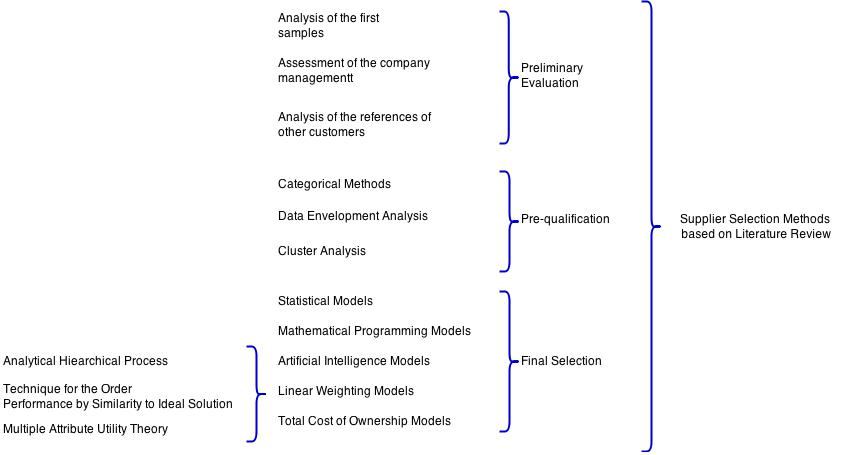
\includegraphics[width=1\textwidth]{Methods.jpg}
  \caption{Suggested division of the methods (Mendoza, 2007)}
\end{figure}

Evaluation of suppliers is supported by ISO normalization – the ISO 9000 series help to evaluate required quality and helps managers mainly in the prime phases of the process.
One of the main objectives of evaluation is getting feedback from the side of the supplier. The right usage of the data can help us to decide whether the supplier is worthy of the partnership, there is some change needed or the company should not continue cooperating. For this reason the companies should keep their database of suppliers updated as much as possible.


\podsekce{Selection of supplier based on quality assessment – ISO 9000}
Evaluation of suppliers is supported by ISO normalization – the ISO 9000 series help to evaluate required quality and helps managers mainly in the prime phases of the process. These standards were designed for companies which want to prove that are capable of consistent production and supply.

Main objectives of the system of quality are (Menšíková, 2009):
  \begin{itemize}
    \item Strict requirements of the purchase should be set
    \item Convenient choice of the supplier
    \item Agreement for the quality safety, including the steps for the solution in the case of conflict in the quality area (usually other standards)
    \item Input checks
    \item Evidence about the quality when the goods are received
  \end{itemize}

\podsekce{Pre-selection process}
The main objectives of prequalification are to effectively eliminate completely or partly inconvenient suppliers and it is rather process of sorting than ranking. (de Boer et al., 2001) T The pre-selection methods helps to make further investigation more comprehensive. Some systems use these methods for final decisions which can lead to infectivity, on the other hand the usage of these methods for final selection is easy and very quick.

\podsekce{Preliminary evaluation}
Nenadál (2006) suggests to make primer selection based on analysis of the first samples, assessment of the company management and references of other customers.
\begin{itemize}
  \item Analysis of the first samples means that the company takes the provided samples and compare them with their own requirements. The company must take into account fact that samples might be produced in completely different environment then standard high volume production. This approach is limited to raw material, stock products, and final products, otherwise the method of the assessment of the company management must be applied.
  \item Assessment of the company management is a process when supplier receives a survey with a focus on prior criteria and is further examined. In case of the Ikea Company, the supplier could expect questions concerning environmental issues, net price or development and modernization.
  \item Analysis of the references of other customers represents experience of other customers with the particular supplier. This approach is not recommended for the final decisions as the requirements differ company from company.

\end{itemize}


\podsekce{Pre-qualification methods of supplier selection}
Among the pre-qualification methods, there are: categorical methods, data envelopment analysis and cluster analysis. (Pal et al., 2013) \par
Categorical system is qualitative model which evaluate historical data and company’s experience with the supplier. First the supplier’s performance is classified as negative, neutral or positive and secondly, based on average rating the supplier receive overall evaluation: negative, neutral or positive. Czech literature (Ochrana, 2004) suggests to divide methods into categories of methods of simple evaluation and methods of weighted evaluation. In this case it is appropriate to involve methods of simple evaluation in categorical system. There are three scales:
\begin{itemize}
\item Nominal scale – the simplest method, which does not carry much information and have two values 0/1, yes/no or convenient/inconvenient. Disadvantage of this method is, that preferences of each criteria cannot be displayed
\item Ordinal scale – compares criteria either by order or by scale points (1-10). The supplier with most points either wins or is further examined.
\item Cardinal scale – expresses how many times or how much is evaluation of one bid higher than the one of the other is. In practice this means that all data has the same denominator and are expressed by percentage. The best supplier stands for 100\% and the rest scores proportionately.
\end{itemize}

Data envelopment analysis (DEA) is a method which put suppliers into two categories, ‘efficient’ and ‘inefficient’ according to the performance of the inputs and outputs. It is a linear programming method which allows to measure multiple criteria at once. The method also gives results which can help to improve partnerships with ‘inefficient’ supplier. The DEA was evaluated as the most popular approach for supplier evaluation. (Weber et al.,xxx) \par

Cluster Analysis (CA) is a basic method from statistics which uses a classification algorithm to group a number of items which are described by a set of numerical attribute scores into a number of clusters such that the differences between items within a cluster are minimal and the differences between items from different clusters are maximal. This classification is used to reduce a larger set of suppliers into smaller more manageable subsets. (Holt, 1998)


\podsekce{Selected systems and models for the final selection of the suppliers}
Most of the designed systems and methods are proposed for the final selection. Also, most of them are multi-criteria decision making approaches (MCDA). The thesis will further discussed the weighted point system which mostly includes the linear weighting models and cost based system which includes total cost of ownership method (TCO) in details. To mention more complex approaches, which are not very popular due to its complicated structure, there are statistical models, mathematical programming models and artificial intelligence models. These models are usually used in larger companies where cost based system is implemented.\par
Statistical models capture the uncertainty related to the supplier selection problem, for example, uncertain demand. As an approach to capture uncertainty, Ding et al. (Ding et al., xxx) proposed a simulation optimization methodology for supplier selection. The methodology consists of three parts: (1) a genetic algorithm (GA) optimizer that continuously searches for new supplier portfolios; (2) using the output from the GA optimizer, a discrete-event simulation model is run to evaluate suppliers on pre-selected key performance indicators (KPI’s); (3) after simulation runs, a fitness value is calculated based on the KPI’s. The fitness is returned to the GA optimizer to search for the next supplier portfolio. Genetic algorithm is a kind of algorithm, which takes inputs which are supposed to be optimized and generate the score, which should be ideal for certain usage. (Mendoza, 2007)\par
Mathematical programming models are very suitable for the supplier selection problem as these models can optimize results using either single or multi objective models. To highlight one example, there is a goal programming model (GPM), which includes decision-maker that is able to process data with set target levels, the goals on different criteria. \par
Artificial intelligence models are models which are able to work with experience and historical data, therefore they can pretend human behavior and decisions. Models are very good at coping with unpredictability and uncertainty which is very often included in the process of supplier selection and at the same time they lack the subjectivity which arises with the human factor.


\podsekce{Weighted point system and linear weighting models}

The system of weighted points is closer to objectivity then the categorical system. Weighted point system places a numerical weight on each criteria and multiples them with these weights. Several issues regarding the system must be understood: the company management must carefully select the most important criteria and decide the weights put on each performance (Monczka et al., 2005). The favorite models for weighted point system are e.g.: Analytical Hierarchical Process (AHP), Technique for the Order Performance by Similarity to Ideal Solution (TOPSIS) or Multiple Attribute Utility Theory (MAUT) \par
AHP was designed by Saaty (1980) and since then was implemented in many different fields such as planning and selecting. The model is based on three principles: structure of the hierarchy, comparative (usually pairwise) judgment of the alternatives and synthesis of the priorities (Amiri, 2010). The hierarchical system has at least three levels. After the decision criteria are put in structure, the pairwise judgment can start from the second level, going to the lowest level. In each level the criteria are compared pairwise according to their levels of influence and based on the specified criteria in the higher level. The judgement are based on the question: ‘How important is criterion A relative to criterion B?‘ In AHP, comparisons are based on nine levels as seen in \par
TOPSIS is a technique based on the concept of distances. Optimal solution, alternative should have the farthest distance from the negative ideal solution and shortest distance from the positive ideal solution. The method includes identifying of the closeness coefficient which determines the ranking order of all suppliers and defining the linguistic values which assess the weights of each criterion. \par
MAUT is a method which mainly differ from AHP and TOPSIS method that can evaluate what-if scenarios. MAUT enables the decision maker to structure a complex problem in the form of a simple hierarchy and to subjectively evaluate a large number of quantitative and qualitative factors in the presence of risk and uncertainty MAUT also handles multiple conflicting factors. The application of the MAUT method involves following steps (Min, 1994):

\begin{enumerate}
  \item Identifying of the “performance matrix” and scope of the problems with the goals.
  \item Defining the criteria and putting them into a “value tree”
  \item Calculation of the relative importance of the criteria
  \item Establishing a relationship between the criteria and the utility scores (attractiveness), putting a utility score on each criterion.
  \item Computing the overall utility score for each decision alternative and rank alternatives in terms of aggregate utility scores.
  \item Perform sensitivity analyses, which describes either the weights are set properly or some changes should be done.
\end{enumerate}


\podsekce{Cost based system and total cost of ownership model (TCO)}
The cost based system is considered to be least subjective. The system quantify the total cost and considers that the lowest buying price does not mean lowest total price. Part of the evaluation is the estimation of the additional cost. Companies often calculate a supplier performance index (SPI), which shows the level of satisfaction (best result is 1) with each item/commodity provided by the supplier.
\newline
$$SPI = \frac{Total \: purchases + Nonperformance \: Costs}{Total \: Purchases}$$
\newline
This approach requires identifying of costs beyond the purchase, which usually includes unit price, transport and tooling. Formally the TCO is defined as the present value of all costs associated with a product, service, or capital equipment that are incurred over its expected life. Costs can be broken into four broad categories:


\begin{itemize}
\item Purchase price – the amount paid to the supplier.
\item Acquisition costs – all costs connected to the process of bringing the product (including the taxes and administration.
\item Usage costs – costs associated with the processing of the material/part into the finished product. This involves for example inventory, scrap, warranty claims and others.
\item End-of-life costs – all costs which must covered after the product reaches the end of the lifespan. Examples are costs linked to obsolescence, disposal or clean up.
\end{itemize}


Introduction of the TCO model can be in many case a very difficult task which requires input from different departments within the company. The company management must be insured that all costs were captured correctly through the entire life cycle. Also the accounting systems are not designed to include nonperformance costs (Monczka et al., 2007) The wood industry is a convenient business for implementing TCO model as the costs connected to the process of wood can be extremely high.




\kapitola{Practical part}

The practical part of the bachelor thesis analyzes the current system of supplier evaluation. The first part deals with the introduction of the company and enterprise. The follow-up section summarize the past evaluation system and tries to describe the biggest disadvantages of the past system and finally the work is focused on the current system and analyze individual criteria with the help of the literature review and of the employees of the Malacky’s enterprise. \par
All numbers included are real but the names of suppliers are replaced with the letters.

\sekce{Company and enterprise introduction}
The main concept of IKEA is to offer good quality for reasonable prices and to the many people. Behind good quality there are features as good function, design and value, everything done with respect to the sustainability. The IKEA was founded by Ingvar Kamprad in 1947 and the company names is an acronym: I and K are initials of the founder and E and A are the first letters from the names of the farm and village where he grew up - Elmtaryd and Agunnaryd. \par
The IKEA stores work under the franchise agreement and the stores are located worldwide with the main quarters in the Netherlands with total sales in 2014 of 28.7 billion of euros. \par
IKEA’s main vision is: “To create a better everyday life for the many people” and “to offer a wide range of well-designed, functional home furnishing products at prices so low that as many people as possible will be able to afford them” is the business idea and IKEA tries to fulfill this through constant optimizing the value chain, good partnership with suppliers, investing in highly automated production and producing large volumes.

\podsekce{doplnit}
IKEA intern directives follows certain rules in choosing potential suppliers. It was first set in 2000 to protect company’s reputation and mainly to actually prevent destroying the environment. IWAY directives (2012) comprised following sections:
\begin{itemize}
  \item Start-up Requirements, IWAY Musts – requirements which must be compiled before signing any contract. This point includes description of  child and forced work, insurance, wages, severe safety hazards and environmental pollution
  \item General Conditions
  \item Environment – Air, Noise, Water and Ground
  \item Chemicals
  \item Hazardous and Nonhazardous Waste
  \item Fire Prevention
  \item Worker Health & Safety
  \item Housing Facilities
  \item Wages, Benefits and Working Hours
  \item Child Labour
  \item Forced & Bonded Labour
  \item Discrimination
  \item Freedom of Association
  \item Harassment, Abuse and Disciplinary Actions
\end{itemize}


The IWAY Forestry Standard - part of the IKEA supplier code of conduct, sets out the minimum criteria for all wood and board supplied to IKEA:

\begin{itemize}
  \item Not from forests that have been illegally harvested
  \item Not from forestry operations engaged in forest-related social conflicts
  \item Not harvested in geographically identified Intact Natural Forests (INF) or High Conservation Value forests, unless they are certified as responsibly managed
  \item Not harvested from natural forests in the tropical and subtropical regions being converted to plantations or non-forest use
  \item Not from officially recognized and geographically identified commercial genetically modified (GM) tree plantations.
\end{itemize}

Suppliers must have procedures in place to implement these standards throughout their supply chain and be able to track and report the origin of their wood.
Forest Stewardship Council standards vary from country to country depending on the type of forest, local conditions and stakeholder interests, but are guided by a set of common principles and criteria determined by the FSC’s members. Among other things, they aim to:

\begin{itemize}
  \item Protect biodiversity
  \item Ensure forest regrowth
  \item Protect the rights and needs of people who work and live in the forest
  \item Stimulate economic development.
\end{itemize}

\podsekce{5.1.2. IKEA and suppliers}

For IKEA it is very important that potential suppliers share the same ideas about business. This means long term partnership, everyday performance, constant development and making profits on high volumes rather than on high margins – reducing overhead costs, better logistics, better supplier purchase and production process and many others. IKEA also tries to bring closer the needs of customers and possibilities of suppliers with continuous evaluation of real life situations as seen in the Fig 4.


\begin{figure}[ht!]
  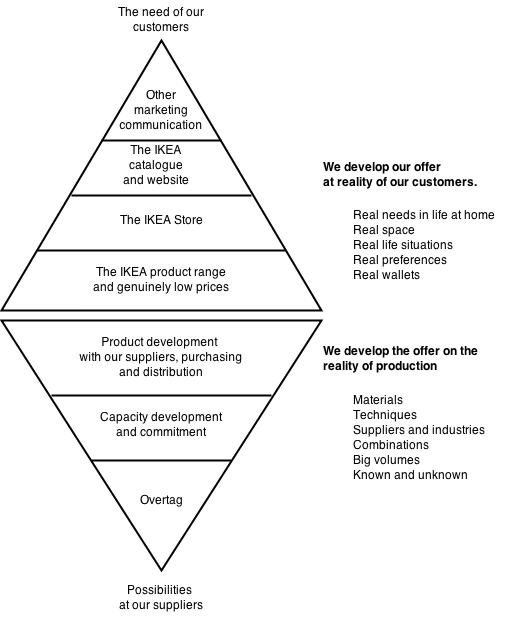
\includegraphics[width=0.8\textwidth]{IKEA_business_model.jpg}
  \caption{IKEA business model}
\end{figure}


\podsekce{IKEA Industry}

IKEA Industry is a group of subsidiary companies, fully integrated international industrial group of IKEA. There are 44 production units in 11 countries.
The role of IKEA Industry is to:
\begin{itemize}
  \item Create outstanding customer value in terms of price and quality.
  \item Create capacity for growth in strategic important categories where capacity is hard to find or there is a monopoly/oligopoly situation.
  \item Add production competence to IKEA and suppliers find or there is a monopoly/oligopoly situation.

\end{itemize}


\sekce{Analysis of the past evaluation system}
The last system of evaluation of suppliers was designed by the former SWEDSPAN Company, currently IKEA Industry. The system was inconvenient for several reasons, but the most importantly the level of objectivity was very low. Processes, inputs and outputs are described in the flowchart in the appendix.

Operations involved:

\begin{enumerate}
  \item Surveys, which required to be filled and sent back, are sent to chosen suppliers.
  \item Evaluation of the surveys, the ones which were assessed as inconvenient are excluded, the ones who passed are asked for samples.
  \item Samples are assessed, based on IKEA requirements IOS – MAT – 0003, 010, 066, 069  and the REACH requirements
  \item Testing of the samples, manager of the production makes a written transcript and send it to the business manager and controlling manager
  \item Technical specifications received from customers are dealt through process PP04.01 and request for price list is made based on quality and quantity requirements
  \item   Inconvenient price offers are excluded
  \item Material files, IKEA requirements (environmental issues, IWAY) and sample tests are archived and samples are placed in a laboratory. Manager of quality and environment is responsible
  \item Results of testing forms a base for internal discussion. Business manager, manager of production and manager of quality and environment are present. Comments are sent to business manager
  \item Business manager in cooperation with manager of production choose strategic and substitute supplier based on available information
  \item Realization of the purchase of products and services.
  \item Revaluation of suppliers based on set criteria, category assessment – strategic or substitute supplier
  \item Archiving of the evaluation
  \item Internal decision about audit, if necessary, the action is followed by supplier audit
  \item The audit is made before the first supply and the results are archived in business department

\end{enumerate}


\podsekce{Methodology of evaluation of suppliers in the past evaluation system}

Each part of the evaluation was given point value as follows:

\begin{itemize}
  \item Point scale 1-3: terms of delivery, price, on time deliveries, warranty claim reactions
  \item Point scale 1-3 and 5: wood kind (5 is a classification for recycled wood)
  \item Point scale 1, 3, 5:  dependency on the supplier, product range (processing expenses)
\end{itemize}

\podsekce{Disadvantages of the past system}
According to responsible person in the enterprise, main disadvantages of the system were spotted in the low objectivity. No further specification for evaluation were given, so in case of evaluating where more than one person was involved, there was an occurrence of disagreement. Person responsible for evaluating of the wood supplies in the Slovak Republic did not have the same ideas about evaluating of the suppliers as the person who did evaluation in the region of the Czech Republic. Also the cost of transport from different places then in the Slovak Republic moved the suppliers from different countries to the bottom of the scale.

\sekce{Current supplier classification – evaluation system}
The document describes the methodology and process for how to perform the Supplier Classification. The purpose with supplier classification is to structure the supplier base according to the following criteria: strategic fit, track record of performance (based on 4 best buy criteria) and how dependent IKEA is on the supplier. The supplier classification will secure a common view on the performance of the supplier base and support identification of potential areas of improvement at the suppliers. \par
Currently, the method is applicable only for classification Home Furnishing Suppliers and Components Suppliers and this thesis suggests possible improvements for application in the IKEA Industry (in Malacky)\par
IKEA classify the supplier base based on long term performance, strategic fit and how dependent IKEA is on the supplier \par
IKEA drives supplier development focusing on capability and strategy to develop future performance – these dimensions + potential other criteria that are viewed as critical to develop the business are in focus of the supplier evaluation.


\podsekce{Working Method}
The method describes step by step how to manage supplier evaluation. All the data are inserted into Excel table.


\begin{description}
  \item[Step 1: Select suppliers to be classified] \hfill \\
  The principle is that all active suppliers shall be classified and each supplier’s performance shall be evaluated and scored individually. If the supplier is part of a group of companies, strategic fit and product development/innovation shall reflect the group of companies (where applicable). If a supplier is decided to be on exit no classification needs to be done. \par
  For suppliers with very small notified volumes (one-time buys etc.) in combination with the supplier is of low importance to IKEA, a classification is not needed. \par
  The reasons for not classifying certain supplier need to be defined, documented and presented as part of the approval of the classification. \par
  In case of shared suppliers between different entities, secure dialogue around supplier performance and business importance in the different entities and agree on which entity that shall classify the supplier taken into account the complete performance picture of supplier.


  \item[Step 2: Define criteria/reference point] \hfill \\
  Collect the agreed goals and wished position (where applicable) for the supplier classification criteria. If relevant, define the category specific criteria (1 or 2) including defining the thresholds for scoring (from 1 to 4).\par
  A category specific criteria can only be added if it is crucial for performance in the specific category. \apr
  Wished position is the lowest possible position in criteria lowest price and product quality. Category goal the position which should be actually achieved or slightly exceeded by the best suppliers.\par
  Open Supplier Classification Tool and insert the goals and wished position for the defined criteria and load; suppliers, notified volumes for previous year and track record of performance. Make sure all suppliers within the category have been loaded, if not, insert the missed out supplier´s and their data manually. In our case all data will be inserted manually

  \item[Step 3: Score and Classify Suppliers] \hfill \\
  Review the loaded performance data on all suppliers. If there has been any external factors impacting the performance of the supplier(s) (e.g. radical increase in raw material prices affecting the price development) the performance can be manually adjusted to compensate for such events. Any manual correction need to be documented in the supplier classification tool with a reason. \par
  Scoring on the different criteria will be performed automatically based on the loaded data. The exceptions are the category specific criteria where is needed to perform the scoring based on set reference points (1-4). \par
  Once the performance scoring is complete perform the following evaluations for each supplier:
  \begin{itemize}
    \item Evaluate the strategic fit between the supplier and IKEA
    \item Evaluate if it is a potential product development/innovation supplier. If yes, perform the detailed evaluation of the supplier
    \item Type in the latest IWAY approved status (Yes/No)
    \item Evaluate how dependent IKEA is on the Supplier.
  \end{itemize}

  Once all performance data is complete and the evaluations mentioned in 3.2 are performed and result inserted in the supplier classification tool on all suppliers, a proposed classification can be calculated by clicking the button “calculate proposed classification”. \par
  Supplier with track record only for 1 or 2 years, the average of the performance will be calculated based on the track record over time that is available. If track record is less than 3 years it is not possible to become IKEA Prioritized supplier. \par
  Evaluation tables can be found in the appendix.

  \item[Step 4: Create total picture through] \hfill \\
  \begin{itemize}
    \item Dialogue with business development teams to create a common picture around performance and improvement areas
    \item Category Manager/Category Leader (Components) to share good examples/ benchmarks
  \end{itemize}

  \item[Step 5: Summarize Supplier Classification through] \hfill \\
  \begin{itemize}
    \item Dialogue to conclude on classification for suppliers in several categories/entities. Guidelines for “hierarchy” of classification is:
      \begin{itemize}
      \item IKEA Critical Supplier
      \item IKEA Prioritized Supplier
      \item IKEA Potential prioritized Supplier
      \item IKEA Product development/Innovation Supplier
      \item IKEA Supplier
      \end{itemize}
    \item Summarize classification and motivations for deviations (if applicable)
    \item Present in category council for approval.
    \item Update and save supplier classification tool with final approved classification for each Supplier based on decision in category council. This shall be done latest one week after approval in category council

  \end{itemize}
  \item[Step 6: Communicate and follow up on Supplier Classification ] \hfill \\
  In the APL process, the following shall be secured:
  \begin{itemize}
    \item Supplier Classification is communicated to the Supplier, including the logic why they have a certain Classification
    \item Correct resources are allocated to the Supplier according to the principles:
    \item Senior competence for Prioritized suppliers
    \item Minimum in the role for Critical, Product development/Innovation and Potential prioritized suppliers
    \item Clear link to Supplier Classification, e.g., critical supplier have plan to fix performance issues, potential prioritized should have APL to close gap to prioritized
  \end{itemize}
  In cases of changed classification, always communicate the driver for the change together with the new classification to the supplier and relevant internal stakeholders.

\end{description}


\sekce{Analysis of individual criteria from the current evaluation system}

Criteria indicated in the Tab. 2  are the ones which requires either both – wished position and category goal or just category goal

% tab 2
\begin{table}[h]
  \tiny
  \begin{tabular}{lllll}
    Criteria                               & Wished Position &  &  & Goal \\
    Lowest price (Current PuA)             &                 &  &  &      \\
    Price development (PuA)                &                 &  &  &      \\
    Product Quality (COPQ)                 &                 &  &  &      \\
    Quality development (COPQ)             &                 &  &  &      \\
    Availability – On time delivery sender &                 &  &  &      \\
    &                 &  &  &      \\
    Supplier Sustainability Index          &                 &  &  &      \\
    Category specific 1*                   &                 &  &  &      \\
    Category specific 2*                   &                 &  &  &
  \end{tabular}
\end{table}

The original new supplier evaluation table can be found in the appendix.
Scale of evaluation: 1-4 according to below thresholds.
>10\% deviation from category goal = 1
Below category goal, max 10\% deviation from category goal = 2
Below wished position or according to category goal = 3
According to wished position or above = 4

If the scale differs, it will be written in the specific criteria description.

\podsekce{Strategic Fit}
Strategic fit shows overall understanding of the supplier. To avoid subjectivity it is strongly recommended to leave a comment why supplier scored the certain point evaluation. Suppliers can receive 1-4 point in each part. Strategic fit further includes following topics:
\begin{itemize}
  \item Business model
  \item Values
  \item Others
  \item Growth
  \item Organization and competence
\end{itemize}

Specification for each topic can be found in appendix. \par
Weight: 6,25\%



\podsekce{Lowest Price (Current PuA)}
Description: Price benchmark between existing suppliers towards wished position and goal within the category/segment. Lowest price (PUA) can be considered on a regional basis if relevant (e.g., in cases of high transportation cost). \par
Weight: 25\% \par

To complete this step of evaluation there we needed to set material categories, because IKEA Industry in Malacky processes more than one kind of material. \par
Next, the prices differ with every supplier. For this reason there are two main ways which are included in the suggested model. Free Carrier (FCA) price is a price without the transport and Delivered at Place (DAP) price which includes the transport costs. \par
The data were transferred to the evaluation table as follows:

\begin{enumerate}
  \item Category goal and wished position were set for each category
  \item Each supplier was evaluated in the categories of delivered material, some in both FCA and DAP section, some of the suppliers only in DAP when the cost of transport was not known
  \item If the prices differ, the average price was taken into account
  \item The results for each supplier were averaged
\end{enumerate}

Price development was also suggested to be the most important criteria from all the mentioned.


\podsekce{Price development (PuA)}
Description: Average ongoing price development compared to average category goal over the past 3 full years. \par
Weight: 25\% \par
The criteria description was further discussed and the final decision was to evaluate the price development based on the track of the difference between ongoing price and price of the commodity index

\podsekce{Product quality (COPQ)}

Description: Benchmark between existing suppliers towards wished position and goal within the category/segment on COPQ.\par
Weight: 6,25\% \par
The criteria was specified as the ratio between the whole volume and the volume with costs connected to the poor product quality. The problem should be further discussed as sometimes the volume does not say much about the actual problem, so the price should be included as well.


\podsekce{Availability – On time delivery sender}
Description: Dispatch precision is based on Notified on time by the supplier versus Ordered value per supplier and week. An average of the last 52 weeks shall be base for the evaluation. \par
Weight: 6,25\% \par
For the purpose of the usage in IKEA was suggested to use data of fulfillment according the contract, which divides year into the quarters.

\podsekce{Sustainability index}
We did not include the index in the evaluation system. The criteria MSS (Main sustainable sources), which shows percentage of using certified forests, and Sustainability, showing the overall supplier approach to the energy, water and waste management, were added instead. \par
Weight (MSS): 12,5\% \par
Weight (Sustainability): 18,75\% \par

\podsekce{IWAY Approved}
If the supplier is not classified as approved, the company should be automatically classified as the critical supplier. For the purpose of IKEA Industry in Malacky, there has been a suggestion to narrow this down to the IKEA must, the first chapter in the IWAY directives.

\podsekce{Product development/Innovation}

If the supplier is classified as innovative is further evaluated in the following topics:
\begin{itemize}
  \item Innovation capability
  \item Vitality
  \item Develop on factory floor
  \item Tools and documentation
\end{itemize}
The classification includes detailed description for evaluating each category. Nevertheless current suppliers do not show much of the intentions for the innovation or development, so the criteria are not further discussed.


\podsekce{IKEA Dependency}
The reason for defining how dependent IKEA is on a supplier shall be based on reasoning around the answers to the following questions:

\begin{description}
  \item[Is it possible to replace or cancel the range delivered by the supplier? ] \hfill \\
  If not possible to replace or cancel the range it will support a high dependency score (3-4) and vice versa.

  \item[How long time would it take to move to an alternative supplier? ] \hfill \\
  For complex products requiring long start up process, or where limited/none alternative suppliers exists today it supports a high dependency score (3-4) and vice versa.

  \item[What is the cost of moving to an alternative supplier?] \hfill \\
  In case of high cost of moving to a new supplier, the decency shall be considered as high (3-4) and vice versa.

\end{description}

For the usage in the enterprise we had to develop quite a different evaluation system. We decided to include volume dependency, price and patent.


\begin{figure}[ht!]
  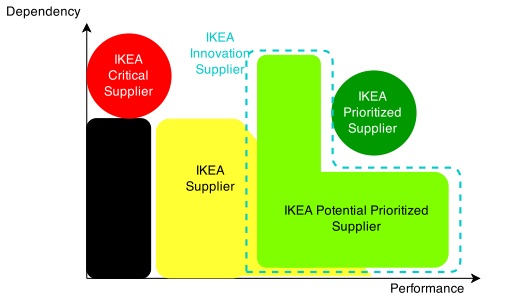
\includegraphics[width=1\textwidth]{vykres.png}
  \caption{IKEA dependency matrix}
\end{figure}

\sekce{Classification}

According to the results, suppliers are classified as indicated in Tab. 3.

% tab 3

\begin{table}[h]
  \tiny
  \begin{tabular}{|l|l|}
    \hline
    \textbf{Classification}                                                                        & \textbf{Scoring condition}                                                                                                                                                                                                                      \\ \hline
    \begin{tabular}[c]{@{}l@{}}IKEA Prioritized \\ Supplier (P)\end{tabular}                       & \begin{tabular}[c]{@{}l@{}}IWAY approved is Yes, Strategic fit score ≥ 3, \\ IKEA dependency score ≥ 3, \\ Long high stable Performance score ≥ 3.\end{tabular}                                                                                   \\ \hline
      \begin{tabular}[c]{@{}l@{}}IKEA Potential \\ prioritized Supplier (T)\end{tabular}           & \begin{tabular}[c]{@{}l@{}}IWAY approved is Yes, Strategic fit is scoring ≥ 3 \\ and Performance scoring is \textgreater2, if new \\ supplier no track record is needed. \\ New supplier can be classified as Potential prioritized.\end{tabular} \\ \hline
        \begin{tabular}[c]{@{}l@{}}IKEA \\ Product development/\\ Innovation Supplier (I)\end{tabular} & \begin{tabular}[c]{@{}l@{}}IWAY approved is Yes, Product development \\ and Innovation is Scoring ≥ 3, \\ No big Performance issues, scoring \textgreater1,5.\end{tabular}                                                                        \\ \hline
          IKEA Supplier (S)                                                                            & \begin{tabular}[c]{@{}l@{}}IWAY approved is Yes. Suppliers that does not fulfill the \\ criteria for any other Supplier classification and total \\ business with IKEA \textless 20 MEUR and \textless 10 \% \\ of the category\end{tabular}      \\ \hline
          \begin{tabular}[c]{@{}l@{}}IKEA Critical \\ Supplier (C)\end{tabular}                          & \begin{tabular}[c]{@{}l@{}}One or more of following criteria; IWAY approved \\ No or Performance score is low, combined with high \\ IKEA dependency scoring ≥3.\end{tabular}                                                                     \\ \hline
          \end{tabular}
        \end{table}


\podsekce{Changes and suggestions to the original new evaluation system}
The analysis of the evaluation system led to the following suggestions:


\begin{itemize}
  \item Considering the weight distribution. The weights were distributed based on the personal feeling which means that the level of subjectivity is very high. Distributing weights according the AHP model (described in the literature review) is shown in the Tab. 4 and Tab. 5. This is only suggestion for further review.


  % ditable

  \begin{table}
    \scalebox{0.7}{
    \parbox{.50\linewidth}{
    \centering
    \begin{tabular}{l|l|l|l}
      \multicolumn{2}{l|}{Category} & Priotity & Rank \\ \hline
      1     & Lowest Price          & 28.5\%   & 1    \\
      2     & Price Development     & 28.5\%   & 1    \\
      3     & Product Quality       & 5.3\%    & 5    \\
      4     & On Time Delivery      & 5.3\%    & 5    \\
      5     & MSS                   & 11.8\%   & 4    \\
      6     & Sustainabilty         & 20.4\%   & 3
    \end{tabular}
    \caption{Foo}
    }
    \hfill
    \parbox{.80\linewidth}{
    \centering
    \begin{tabular}{l|cccccc}
      & 1                         & 2                         & 3                         & 4                         & 5                         & 6                      \\ \hline
      1 & \multicolumn{1}{c|}{1}    & 1.00                      & 4.00                      & 4.00                      & 3.00                      & 2.00                   \\ \cline{2-3}
      2 & \multicolumn{1}{c|}{1.00} & \multicolumn{1}{c|}{1}    & 4.00                      & 4.00                      & 3.00                      & 2.00                   \\ \cline{3-4}
      3 & 0.25                      & \multicolumn{1}{c|}{0.25} & \multicolumn{1}{c|}{1}    & 1.00                      & 0.33                      & 0.20                   \\ \cline{4-5}
      4 & 0.25                      & 0.25                      & \multicolumn{1}{c|}{1.00} & \multicolumn{1}{c|}{1}    & 0.33                      & 0.20                   \\ \cline{5-6}
      5 & 0.33                      & 0.33                      & 3.00                      & \multicolumn{1}{c|}{3.00} & \multicolumn{1}{c|}{1}    & 0.50                   \\ \cline{6-7}
      6 & 0.50                      & 0.50                      & 5.00                      & 5.00                      & \multicolumn{1}{c|}{2.00} & \multicolumn{1}{c|}{1} \\ \cline{7-7}
    \end{tabular}
    \caption{Bar}
    }
    }
  \end{table}



  \item The introducing part of the table was adjusted to the needs of the IKEA Industry as following:

    \begin{itemize}
      \item Supplier number: number in the database.
      \item Supplier name: official supplier name.
      \item Supplier state (location): supplier country of origin.
      \item Total notified segment current FY (\euro): total production in the certain category (our case: pine/spruce)
      \item Related country notified segment FY (\euro): total production in the specific country
      \item Total notified supplier current FY-1 (\euro): total production of the supplier in the past year.
      \item Supplier share related country FY (in \%): the share of production in the related country.
      \item Main supplied material/component: material which supplier can provide.
    \end{itemize}
    Supplier involvement other segments:
    In the criteria of the lowest price we had to divide the categories of different materials, suggested merged categories are shown in Tab. 5.

    \item Also the evaluation is divided into two main parts: price FCA and DAP. Some suppliers can be evaluated in both, the rest only in DPA
    \item We did not evaluate product quality development.
    \item MSS/Sustainability – these two criteria were added as sub-criteria to the Sustainability index, which was later deleted as we do not know the indexes. MSS (Main sustainable sources) gives a percentage of wood which has been mined in certified forests. Sustainability expresses the overall approach of the supplier to the sustainability- water, energy, and waste management. MSS is expressed in percentage (1-100\%), sustainability 1-4.
  \item IKEA dependency will be evaluated from the point of volume, price and range of supplied materials.
  \item If the IKEA Approved will be classified as no, it will not mean that the supplier is immediately classified as critical. Also other criteria will be assessed.
  \item The classification always round the final results down. This can sometimes lead to the inaccuracies in the classifying. We suggest to further look at the point evaluation in the final step.
  \item The system does not consider processing costs, which can be sometimes very high. The consideration of adding the criteria would be appropriate.

\end{itemize}

\sekce{Comparing and contrasting of the past and new evaluation system}

After the analyzing the system and changing the evaluation system to the needs of IKEA Industry in Malacky, we tried the new system with 15 suppliers from different countries in the region, private and state, small and bigger. In the Tab. 7 we can see results according the past evaluation system and in the Tab. 8 according the new one. Complete tables can be found in the appendix. \par

% tabs
\begin{table}[h]
  \tiny
  \begin{tabular}{c|c|ccc}
    & OLD    & \multicolumn{3}{c}{NEW}                                                                                                                                  \\ \hline
    Supplier & Points & Performance & \begin{tabular}[c]{@{}c@{}}IKEA \\ Dependency\end{tabular} & Approved Classification                                                        \\ \hline
    A        & 20     & 2           & 4                                                          & IKEA Critical Supplier                                                         \\
    B        & 15     & 2           & 2                                                          & \begin{tabular}[c]{@{}c@{}}IKEA Potential \\ Prioritized Supplier\end{tabular} \\
    C        & 24     & 1           & 2                                                          & IKEA Supplier                                                                  \\
    D        & 14     & 1           & 2                                                          & IKEA Supplier                                                                  \\
    E        & 14     & 2           & 2                                                          & IKEA Supplier                                                                  \\
    F        & 19     & 1           & 2                                                          & IKEA Supplier                                                                  \\
    G        & 19     & 2           & 2                                                          & IKEA Supplier                                                                  \\
    H        & 18     & 1           & 2                                                          & IKEA Supplier                                                                  \\
    I        & 21     & 2           & 2                                                          & IKEA Supplier                                                                  \\
    J        & 18     & 1           & 2                                                          & IKEA Supplier                                                                  \\
    K        & -      & 2           & 2                                                          & IKEA Supplier                                                                  \\
    L        & 16     & 1           & 2                                                          & IKEA Supplier                                                                  \\
    M        & -      & 2           & 2                                                          & IKEA Supplier                                                                  \\
    N        & -      & 2           & 2                                                          & IKEA Supplier                                                                  \\
    O        & 17     & 2           & 2                                                          & IKEA Supplier
  \end{tabular}
  \caption{popisek}
\end{table}

\newline
Supplier A is in the TOP 3 suppliers considering the volume. In the past system scored 20 points, which was considered as above average. In the new evaluation system, the supplier was classified as critical. The reasons are the high dependency, which is in the new system seen as rather negative and low MSS/ Sustainability. In the past system the dependency criteria  gave plus points. Further cooperation will continue, but IKEA will probably have more demands in the field of environmental issues such as mining the certified forests. \par
Supplier B does not supply the same amounts as the A supplier, but mined forests are 100\% certified and supplier tends to approach sustainability issues carefully. Supplier scored only 15 points in the past evaluation. The supplier had/has high processing costs, which are not currently implemented in the new system. \par
Supplier C scored 24 points, which is the highest score in the evaluated selection. Supplier offered good quality material at average price. On the other hand, in the new system is classified as IKEA Supplier, because does not mine certified forests and does not have the best quality performance. This might be the result of subjective evaluation.\par
Suppliers D - N have average score in both evaluation system. This means that except one supplier (G) they do not mine certified forests have and have acceptable or very good prices.Suppliers of the chips - K, O -  have even scored 4 points in price development and lowest price development, but because their approach to sustainability and understanding the IKEA model, they cannot be classified otherwise. Supplier I scored 21 points in the past evaluation system and has the best prices in the category of round wood supplies. Again, the supplier does not mine the certified forests.



\kapitola{Discussion}

Over few last years corporations like IKEA were facing the pressure from the stakeholders, public and government to incorporate more responsible approach to the environmental issues. This main reason among other reasons led to the need of creating the new system of supplier selection and evaluation. \par
The current evaluation system in the IKEA Industry Malacky is an example of linear weighted model, where different criteria have different weight. The system was designed specifically for the company with the consultation of McKinsey & Company. \par
The analysis of the system of the system discovered few imperfections. Some criteria could not be used in the system and some had to be added. Also the criteria had to be reassessed. After analyzing the new evaluation system and adjusting the system to the need of IKEA Industry in Malacky we tried the system on 15 suppliers, we included the private and state suppliers and suppliers from different countries.  \par
Results showed that wood-processing industry is not fully ready to fulfill the requirements for the sustainability, at least in the region of central Europe. For most of the suppliers are quantity and competitive prices the most significant factors. From the comparing of  two approaches we can say that the fact that by the year 2020 IKEA wants to have all suppliers classified as IWAY approved, moved most of the suppliers to worse positions.  \par
The classification is currently designed to be very easy to follow and to be convenient for as many divisions as possible. The fact that the output of the evaluation system is classification in 5 categories does not seem sufficient. The evaluation could also include some of the most important data such as overall performance (not in rounded-off form), dependency or supplied volume to give more comprehensive idea about the supplier. \par
The system could be further improved by trying some more complex method which were mentioned in the literature review. Many of these methods can be tried online with low time demand. \par
Further research in the field of supplier in wood-processing industry could include analysis of the suppliers approaches to environmental issues and motivation for the mining of the certified forests.



\kapitola{Conclusion}

The thesis deals with the topic of suppliers evaluation. Based on the literature review, the first part of the thesis describes the purchasing process and functions. This is followed by the section concerning the suppliers and finally by the selected methods - included methods are either modern and popular or easy to use and understand. The main aim of the literature review was to understand the way of creating and compare the current evaluation system which is used in IKEA Industry in Malacky.




\begin{literatura}
\citace{beran}{Beran, 1994}{\autor{Beran, V.} \nazev{Typografický manuál.}
Náchod: Nakladatelství Manuál, 1994. \\ ISBN 80-901824-0-2}
\citace{csn010166}{ČSN 01\,0166, 1992}{\nazev{ČSN 01\,0166 Nakladatelská
(vydavatelská) úprava knih a~některých daląích druhů neperiodických
publikací.} Praha: Federální úřad pro normalizaci a~měření, 1992}
\citace{csn016910}{ČSN 01\,6910, 1997}{\nazev{ČSN 01\,6910 Úprava písemností
zpracovaných textovými editory nebo psaných strojem.} Praha: Český
normalizační institut, 2004}
\citace{csniso31-0}{ČSN ISO 31-0, 1994}{\nazev{ČSN ISO 31-0 -- Veličiny
a~jednotky. Část 0: Vąeobecné zásady}. Praha: Český normalizační institut,
1994}

\citace{csniso31-11}{ČSN ISO 31-11, 1999}{\nazev{ČSN ISO 31-0 -- Veličiny
a~jednotky. Část 11: Matematické znaky a~značky pouľívané ve fyzikálních
vědách a~v~technice}. Praha: Český normalizační institut, 1999}

\citace{csniso690}{ČSN ISO 690, 1996}{\nazev{ČSN ISO 690 -- Bibliografické
citace. Obsah, forma a~struktura}. Praha: Český normalizační institut, 1996}

\citace{csniso690-2}{ČSN ISO 690\spoj{}2, 2000}{\nazev{ČSN ISO 690-2 --
Informace a~dokumentace -- Bibliografické citace -- Část 2: Elektronické
dokumenty a~jejich části}. Praha: Český normalizační institut, 2000}

\citace{csn7144}{ČSN ISO 7144, 1996}{\nazev{ČSN ISO 7144 Dokumentace --
Formální úprava disertací a~podobných dokumentů.} Praha: Český normalizační
institut, 1996}
\citace{Nohel}{Nohel, 1972}{\autor{Nohel, F.} \nazev{Sazba matematická a
chemická}. Praha: SNTL, 1972}
\citace{on882503}{ON 88\,2503, 1974}{\nazev{ON 88\,2503 Základní pravidla
sazby.} Praha: Vydavatelství Úřadu pro normalizaci a~měření, 1974}
\citace{pop}{Pop, Fléger a~Pop, 1989}{\autor{Pop, P., Flégr, J., Pop, V.}
\nazev{Sazba I~-- Ruční sazba.} Praha: SPN, 1989}
\citace{latzac}{Rybička, 2003}{\autor{Rybička, J.} \nazev{\LaTeX{} pro
začátečníky.} 3. vyd. Brno: Konvoj, 2003}
\citace{TalDipl}{Talandová, 2006}{\autor{Talandová, P.} \nazev{Přístupy ve
zpracování tabulek v~systémech DTP}. Diplomová práce. Brno: PEF MZLU v~Brně,
2006}
\end{literatura}

\end{document}

\prilohy
\priloha{Definice stylu dipp}

{\footnotesize
\begin{verbatim}
%%%%%%%%%%%%%%%%%%%%%%%% dipp.sty
%
%  Styl pro sazbu diplomovych praci, v. 1.21
%  Freeware.
%  Omezeni: Pokud kdokoliv provede jakoukoliv modifikaci,
%           nesmi styl sirit pod stejnym jmenem.
%
%  Jiri Rybicka, 29. 1. 2005
%
%%%%%%%%%%%%%%%%%%%%%%%%
%
%  TEST SPRAVNOSTI KODOVANI (kodovani je PC Latin 2)
%  ---------------------------------------
%  Přílią ľlu»oučký kůň úpěl ďábelské ódy.
%  ---------------------------------------
%  Predchozi vetu musite videt spravne.
%
%%%%%%%%%%%%%%%%%%%%%%%%%%%%%%%%%%%%%%%%%%%%%%%%%%%%%%%%%%%

%%%%%%%%%%%%%%%%%%%%%% Vnořené styly

\input graphics.sty

%%%%%%%%%%%%%%%%%%%%%% Rozměrové parametry

\textwidth 150mm \hoffset -5mm
\textheight 220mm \voffset -5mm
\oddsidemargin 14mm
\evensidemargin 6mm

\tolerance 4000
\widowpenalty 5000
\clubpenalty 5000
\raggedbottom

\parindent 2em

%%%%%%%%%%%%%%%%%%%%%% Fonty

\def\markfont{\normalfont\footnotesize\sffamily}
\def\pgfont{\normalfont\bfseries\sffamily}

%%%%%%%%%%%%%%%%%%%%%% Stránkování

\def\ps@headings{%
       \def\@oddfoot{}%
       \def\@evenfoot{}%
       \let\@mkboth\markboth
       \def\@evenhead{\parbox{\textwidth}{{\pgfont \thepage}
                \hfill{\markfont \leftmark}\smallskip\hrule}}%
       \def\@oddhead{\parbox{\textwidth}{{\markfont
       \rightmark}\hfill{\pgfont \thepage}\smallskip\hrule}}}

\def\ps@plain{%
       \def\@oddhead{}%
       \def\@evenhead{}%
       \def\@evenfoot{\parbox{\textwidth}{\pgfont \thepage}}%
       \def\@oddfoot{\parbox{\textwidth}{\hspace*{\fill}
                   {\pgfont \thepage}}}}

\pagestyle{plain}   % implicitně

%%%%%%%%%%%%%%%%%%%%%% Úvodní stránky

\def\typprace{Diplomová}
\def\bakalarska{\gdef\typprace{Bakalářská}}
\def\skola#1{\gdef\@skola{#1}}
\def\fakulta#1{\gdef\@fakulta{#1}}

\def\titul#1#2#3#4{\thispagestyle{empty}
   \vspace*{-20mm}
   \begin{center}
   {\Large \sffamily \@skola\\[8pt]}
   {\Large \sffamily \@fakulta} \par \bigskip \hrule
   \vbox to 165mm{\vspace*{\fill}
   {\Huge\sffamily\bfseries #1\par}\vskip 10mm
   {\large\sffamily\bfseries \typprace{} práce} \par
   \vspace*{\fill}}\par
   \noindent {\large \sffamily
        \begin{tabular}{@{}l}
        Vedoucí práce:\\ #3\end{tabular} \hfill #2}
   \par \vfill {\large \sffamily #4}\end{center}%
}

\skola{Mendelova zemědělská a lesnická univerzita v~Brně}
\fakulta{Provozně ekonomická fakulta}

\def\prohlaseni#1#2{\cleardoublepage\thispagestyle{empty}\vspace*{\fill}\noindent
      \parbox{\textwidth}{\hspace*{\parindent}#1 \\[15mm]
       #2 \hfill \hbox to 60mm{\tiny\dotfill}}}

\def\podekovani#1{\cleardoublepage\thispagestyle{empty}\vspace*{\fill}#1}

\def\abstract#1#2{\cleardoublepage\vspace*{3cm}{\english
       \noindent {\sffamily\bfseries Abstract}\par\medskip
       \noindent #1 \par \medskip #2}}

\def\abstrakt#1#2{\vspace*{3cm}{\noindent
      {\sffamily\bfseries Abstrakt}\par\medskip
       \noindent #1 \par \medskip #2}}

%%%%%%%%%%%%%%%%%%%%%% Obsah

\def\obsah{\cleardoublepage\tableofcontents\cleardoublepage}

%%%%%%%%%%%%%%%%%%%%%% Oddíly v textu

\def\cislovat#1{\setcounter{secnumdepth}{#1}\setcounter{tocdepth}{#1}}

\renewcommand\section{\@startsection {section}{1}{\z@}%
                   {-3.5ex \@plus -1ex \@minus -.2ex}%
                   {2.3ex \@plus.2ex}%
                   {\normalfont\sffamily\Large\bfseries}}
\renewcommand\subsection{\@startsection{subsection}{2}{\z@}%
                   {-3.25ex\@plus -1ex \@minus -.2ex}%
                   {1.5ex \@plus .2ex}%
                   {\normalfont\sffamily\large\bfseries}}
\renewcommand\subsubsection{\@startsection{subsubsection}{3}{\z@}%
                   {-3.25ex\@plus -1ex \@minus -.2ex}%
                   {1.5ex \@plus .2ex}%
                   {\normalfont\normalsize\sffamily\bfseries}}
\renewcommand\paragraph{\@startsection{paragraph}{4}{\z@}%
                   {3.25ex \@plus1ex \@minus.2ex}%
                   {-1em}%
                   {\normalfont\normalsize\sffamily\bfseries}}
\renewcommand\subparagraph{\@startsection{subparagraph}{5}{\parindent}%
                   {3.25ex \@plus1ex \@minus .2ex}%
                   {-1em}%
                   {\normalfont\normalsize\sffamily\bfseries}}

\def\kapitola#1{\clearpage\section{#1}
     \markboth{\thesection\quad \uppercase{#1}}{\thesection\quad
                                \uppercase{#1}}}
\def\sekce#1{\subsection{#1}\markright{\thesubsection\quad #1}}
\def\podsekce#1{\subsubsection{#1}}

\def\appname{Přílohy}

\def\@samstranapriloh{\clearpage\thispagestyle{empty}
        \vspace*{50mm}\begin{center}
        \normalfont\sffamily\LARGE\bfseries
                 \uppercase{\appname}\end{center}
        \addcontentsline{toc}{section}{\appname}
}

\def\prilohy{\@ifnextchar*{\@prilohy{}}{\@prilohy{\@samstranapriloh}}}

\def\@prilohy#1{#1
        \def\thesection{\Alph{section}}\setcounter{section}{0}}
\let\priloha\kapitola


%%%%%%%%%%%%%%%%%%%%%% Literatura

\def\refname{Literatura}

\renewenvironment{thebibliography}[1]
     {\section{\refname}%
      \markboth{\thesection\quad \uppercase{\refname}}{\thesection\quad
                                 \uppercase{\refname}}%
      \list{\@biblabel{\@arabic\c@enumiv}}%
           {\settowidth\labelwidth{\@biblabel{#1}}%
            \itemindent -2em
            \leftmargin 2em
            \@openbib@code
            %\usecounter{enumiv}%
            \let\p@enumiv\@empty
            \renewcommand\theenumiv{\@arabic\c@enumiv}}%
      \sloppy
      \clubpenalty4000
      \@clubpenalty \clubpenalty
      \widowpenalty4000%
      \sfcode`\.\@m}

\def\@citex[#1]#2{%
  \let\@citea\@empty
  \@cite{\@for\@citeb:=#2\do
    {\@citea\def\@citea{; }%
     \edef\@citeb{\expandafter\@firstofone\@citeb}%
     \if@filesw\immediate\write\@auxout{\string\citation{\@citeb}}\fi
     \@ifundefined{b@\@citeb}{\mbox{\reset@font\bfseries ?}%
       \G@refundefinedtrue
       \@latex@warning
         {Citation `\@citeb' on page \thepage \space undefined}}%
       {\hbox{\csname b@\@citeb\endcsname}}}}{#1}}

\def\@lbibitem[#1]#2{\item []\if@filesw
      {\let\protect\noexpand
       \immediate
       \write\@auxout{\string\bibcite{#2}{#1}}}\fi\ignorespaces}

\def\@cite#1#2{({\let\hbox\relax #1\if@tempswa , #2\fi})}

\def\autor#1{\textsc{#1}}
\def\nazev#1{\textit{#1}}
\def\akol{\rm}

\newenvironment{literatura}{\newpage\begin{thebibliography}{}}%
               {\end{thebibliography}}

\def\citace#1#2#3{% ident., tvar odkazu, údaje
\bibitem [#2]{#1} #3.
}

%%%%%%%%%%%%%%%%%%%%%% Výčty a seznamy
\newdimen\leftmargini
\newdimen\leftmarginii
\newdimen\leftmarginiii
\newdimen\leftmarginiv
\newdimen\leftmarginv
\newdimen\leftmarginvi
\leftmargini=2em
\leftmarginii=2em
\leftmarginiii=2em
\leftmarginiv=2em
\leftmarginv=2em
\leftmarginvi=2em

\def\@listi{\leftmargin\leftmargini
            \parsep \parskip% 4\p@ \@plus2\p@ \@minus\p@
            \topsep \parskip% 8\p@ \@plus2\p@ \@minus4\p@
            \itemsep\parskip}% 4\p@ \@plus2\p@ \@minus\p@}
\let\@listI\@listi
\@listi
\def\@listii {\leftmargin\leftmarginii
              \labelwidth\leftmarginii
              \advance\labelwidth-\labelsep
              \topsep   \parskip%  4\p@ \@plus2\p@ \@minus\p@
              \parsep   \parskip%  2\p@ \@plus\p@  \@minus\p@
              \itemsep   \parsep}

\def\labelenumii{\theenumii)}

\def\@listiii{\leftmargin\leftmarginiii
              \labelwidth\leftmarginiii
              \advance\labelwidth-\labelsep
              \topsep   \parskip%  2\p@ \@plus\p@\@minus\p@
              \parsep   \parskip%  \z@
              \partopsep\parskip%  \p@ \@plus\z@ \@minus\p@
              \itemsep   \topsep}
\def\@listiv {\leftmargin\leftmarginiv
              \labelwidth\leftmarginiv
              \advance\labelwidth-\labelsep}
\def\@listv  {\leftmargin\leftmarginv
              \labelwidth\leftmarginv
              \advance\labelwidth-\labelsep}
\def\@listvi {\leftmargin\leftmarginvi
              \labelwidth\leftmarginvi
              \advance\labelwidth-\labelsep}

%%%%%%%%%%%%%%%%%%%%%% Plovoucí prostředí

\def\figurename{Obr.}
\def\tablename{Tab.}

\def\csfigcap#1{\refstepcounter{figure}\parbox{\textwidth}{\small%
       \figurename{} \thefigure: #1}\addcontentsline{lof}{section}{\figurename{}
       \thefigure: #1}}

\def\csfigcapbez{\refstepcounter{figure}\parbox{\textwidth}{\small%
       \figurename{} \thefigure}\addcontentsline{lof}{section}{\figurename{}
       \thefigure}}

\def\cstabcap#1{\refstepcounter{table}\parbox{\textwidth}{\small%
       \tablename{} \thetable: #1}\addcontentsline{lot}{section}{\tablename{}
       \thetable: #1}}

\def\cstabcapbez{\refstepcounter{table}\parbox{\textwidth}{\small%
       \tablename{} \thetable}\addcontentsline{lot}{section}{\tablename{}
       \thetable}}

\def\obrazek{\begin{figure}[htb]\centering }
\def\obrazekp{\begin{figure}[p]\centering }
\def\endobr#1{\par\medskip\csfigcap{#1}\end{figure}}
\def\endobrl#1#2{\par\medskip\csfigcap{#1}\label{#2}\end{figure}}
\def\endobrbez{\par\medskip\csfigcapbez\end{figure}}
\def\vloztif#1{\input #1 \csname set#1\endcsname}
\def\vlozeps#1#2{\scalebox{#2}{\includegraphics{#1}}}

\def\tabulka#1{\begin{table}[htb]\centering\cstabcap{#1}\par\medskip}
\def\tabulkap#1{\begin{table}[p]\centering\cstabcap{#1}\par\medskip}
\def\endtab{\end{table}}

\def\pole#1#2{{\def\arraystretch{.95}\begin{tabular}{@{}#1@{}}
                 #2\end{tabular}}}

{\catcode`\!=\active
\gdef\vykricnik{\catcode`\!=\active \def!{\hphantom{0}}}
}

%%%%%%%%%%%%%%%%%%%%%% Speciální znaky

\def\spoj{\discretionary{-}{-}{-}}
\def\az{\discretionary{}{\hbox{aľ\ }}{--}}
\def\uvv#1{\symbol{159}#1\symbol{158}}

%%%%%%%%%%%%%%%%%%%%%% konec stylu dipp %%%%%%%%%%%%%%%%%%%%%%%%%%%%%%
\end{verbatim}
}

\priloha{Určení rozsahu této práce}
\label{rozsah}
Vyjdeme ze dvou údajů, zjiątěných měřením dokumentu: počet znaků s~mezerami
a~plocha obrázků v~cm$^2$.

Počet znaků s~mezerami $z$: 92\,490

Plocha dvou obrázků $p$: $47 + 36 = 83$ cm$^2$

Počet AA $v$: $$v=\frac z{36\,000}+\frac p{2\,300} = 2,60\;\hbox{AA}$$

Vyjádříme-li rozsah v~normalizovaných stranách $n$, dostáváme:
$$n=v\cdot 20 \doteq 52\;\hbox{ns}$$

Tato práce má rozsah 52 normalizovaných stran.

Vidíme, ľe počet fyzických stran se blíľí počtu normalizovaných stran, i~kdyľ
je zvolen zcela odliąný formát sazby -- stránky vůbec neobsahují počet znaků
odpovídajících normalizované straně. Z~toho jasně vyplývá, ľe usuzovat na
rozsah díla podle počtu fyzických stran je velmi nepřesné a~zcela zavádějící.
\end{document}
